\subsection{Simulation results}

\paragraph{Binary-continuous data}

We start by considering a mix of binary and continuous variables generated as outlined in Section \ref{sec::setup} to compare our methods against the bridge function approach of \citet{Fan17}. For this purpose, \figref{fig:bench_binary} depicts the mean estimation error $\Norm{\hat{\mathbf\Omega} - \mathbf\Omega^*}_F$ and the AUC for the different estimators under the different $(d,n)$ regimes. We include the following estimators for \(\mathbf\Omega^*\): (1) An oracle estimator (\texttt{oracle}) that corresponds to estimating $\hat{\mathbf\Sigma}^{(n)}$ using the mapping between Spearman's rho and \(\hat\Sigma_{jk}^*\) (Eq. \eqref{spearman_mapping}) based on realization of the (partially) latent continuous data $(\mathbf{Z_1},\mathbf{X_2})$. (2) The bridge function based estimator (\texttt{bridge}) proposed by \citet{Fan17}. (3) The polychhoric and polyserial MLE estimator (\texttt{mle}) proposed in Section \ref{sec::latent_gaussian}. (4) The general mixed estimator (\texttt{poly}) proposed in Section \ref{sec::nonparanormal}. In the left column, we set $f_j(x) = x$ for all $j$, i.e., we recover the latent Gaussian model. In the right column, we set $f_j(x) = x^{1/3}$ for all $j$ to recover the LGCM.


\begin{figure}
    \centering
    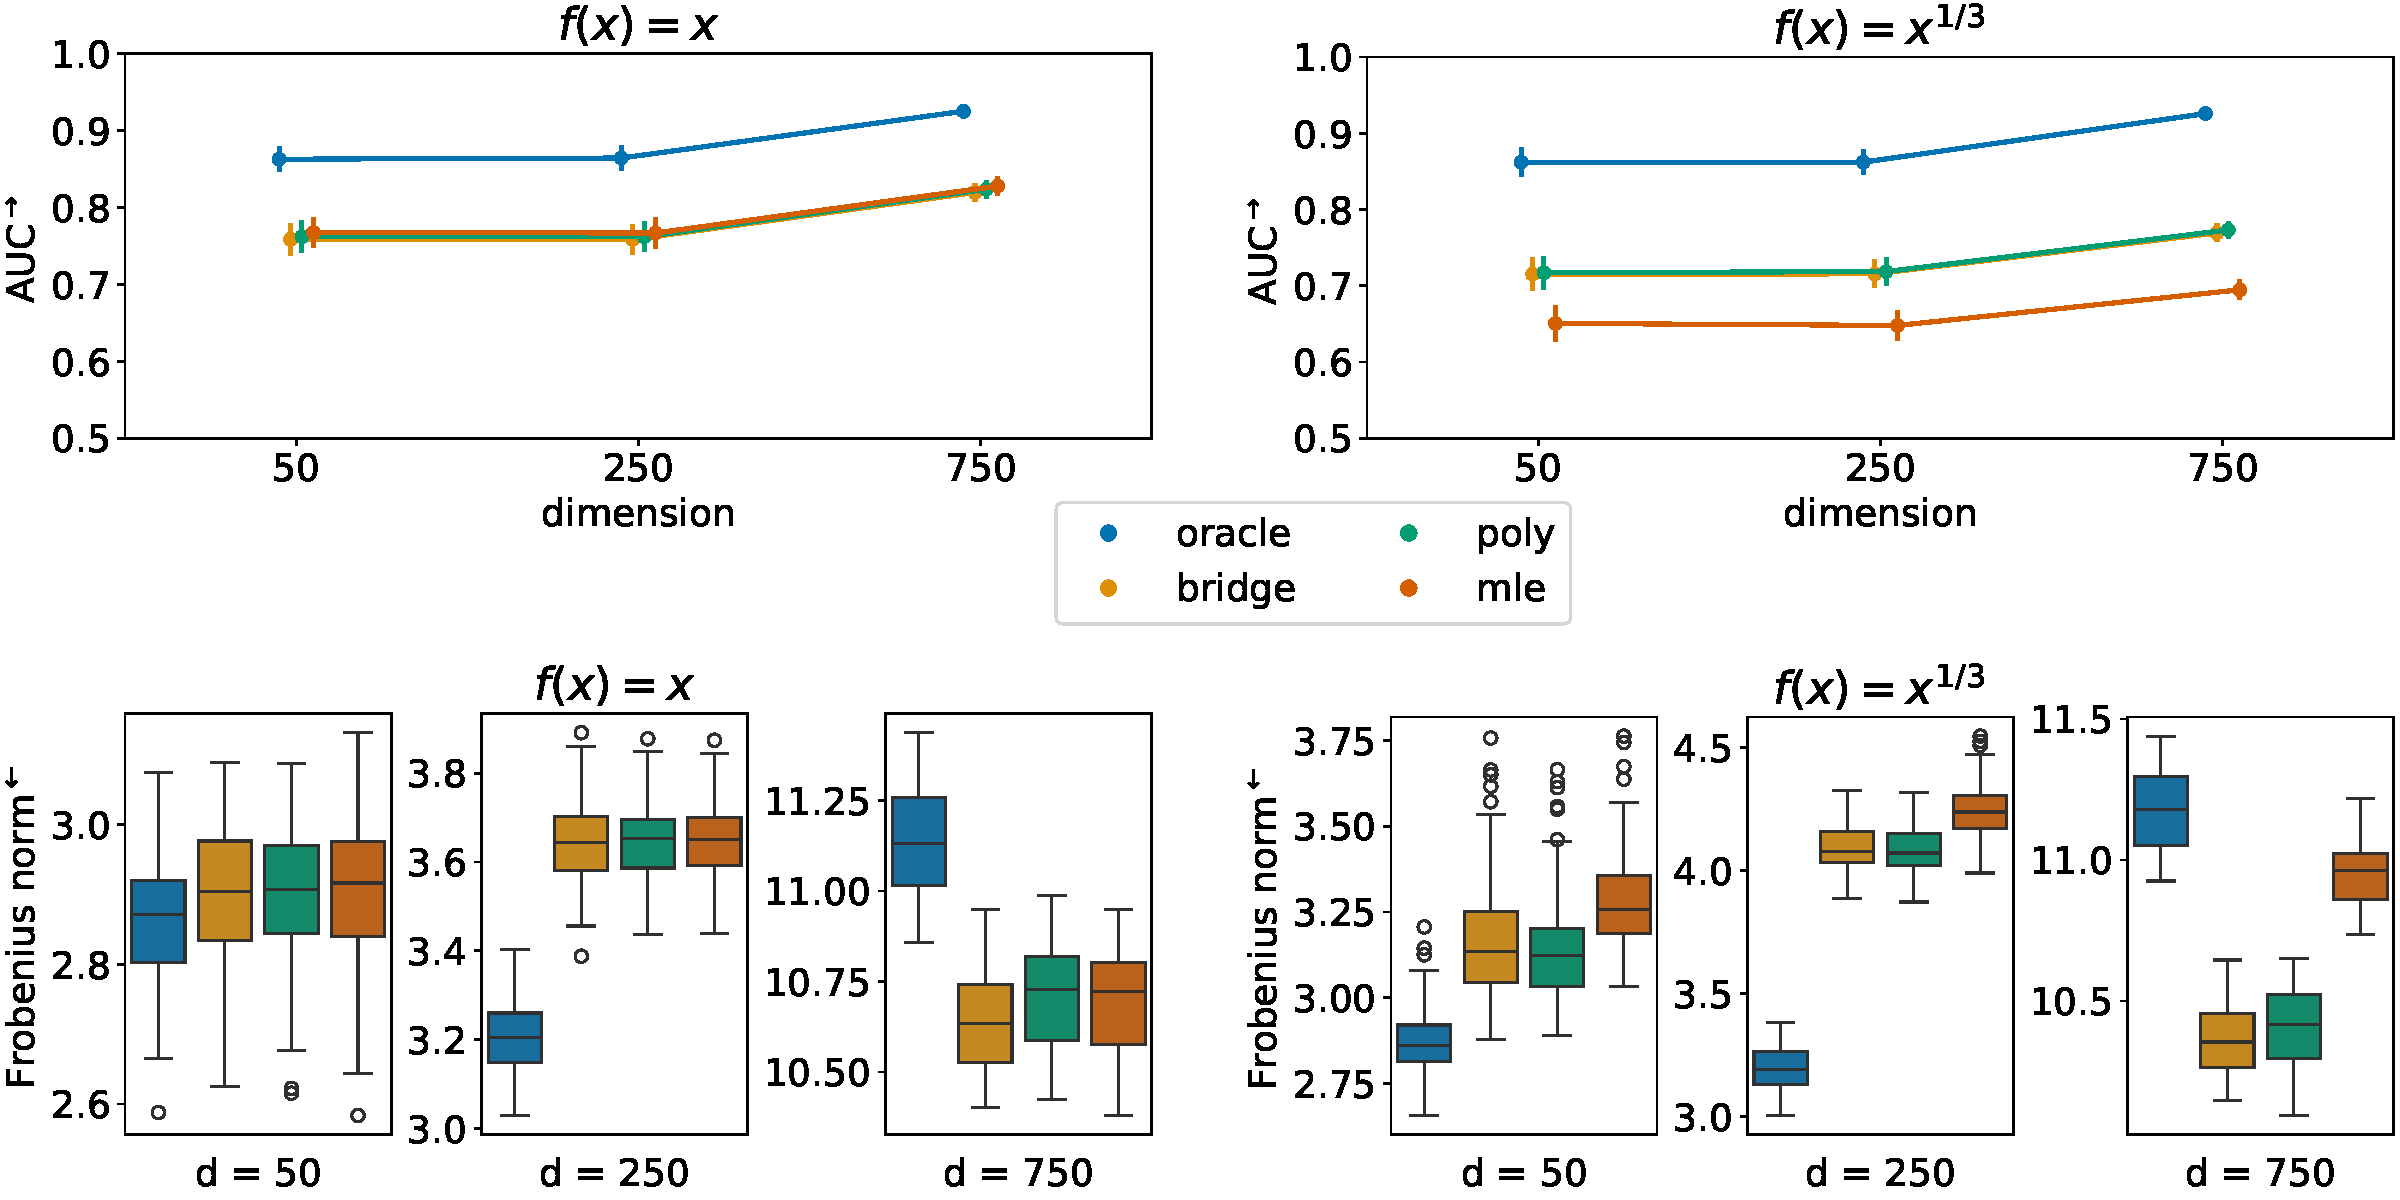
\includegraphics[width=\textwidth]{Figures/simulation_results_binary.pdf}
    \caption{Simulation results for the binary-continuous data setting based on \(100\) simulation runs. The left column corresponds to the latent Gaussian model, where the transformation function is the identity. The right colum depicts results for the LGCM with \(f_j(x) = x^{1/3}\) for all \(j\). The top row reports mean and standard deviation of the AUC along simulation runs, and the bottom row depicts boxplots of the estimation error $\Norm{\hat{\mathbf\Omega} - \mathbf\Omega^*}_F$. The y-axis labels have superscript arrows attached to indicate the direction of improvement: \(\rightarrow\) implies that larger values are better, and \(\leftarrow\) implies that smaller values are better.}
    \label{fig:bench_binary}
\end{figure}

\figref{fig:bench_binary} suggests that under the latent Gaussian model (left column), there are virtually no differences between all non-oracle estimators in graph recovery or estimation error. As expected, the \texttt{oracle} has the highest AUC and lowest estimation error across scenarios. The only exception is the estimation error when the dimension is \(d = 750\). This surprising result stems from an increased FPR for \texttt{oracle} (see Figure 3 in the Supplementary Materials) when minimizing the eBIC with the additional penalty set to $\theta = 0.5$. A higher penalty seems appropriate in this case. Meanwhile, the non-oracle estimators are more conservative, and the additional penalty appears to be chosen correctly in these cases.

In the right column of \figref{fig:bench_binary}, binary-continuous mixed data is generated from the LGCM. The \textit{Case I} and \textit{Case II} MLEs are misspecified in this case, which translates to lower AUC and higher estimation error.
The remaining estimators are unaffected by the transformation. Encouragingly, we find no substantial performance difference between the bridge function approach and our procedure in any of the metrics considered, including the TPR and FPR results in Figure 3 in the Supplementary Materials.

\paragraph{General mixed data}
Let us turn to the general mixed setting. While the bridge function approach by \citet{Fan17} does not extend beyond the binary-continuous mix, we can still compare our approach to the ensemble method developed by \citet{Feng19}. Due to its close connection to the original method, we continue to denote the proposed ensemble estimator \texttt{bridge}.
\begin{figure}
    \centering
    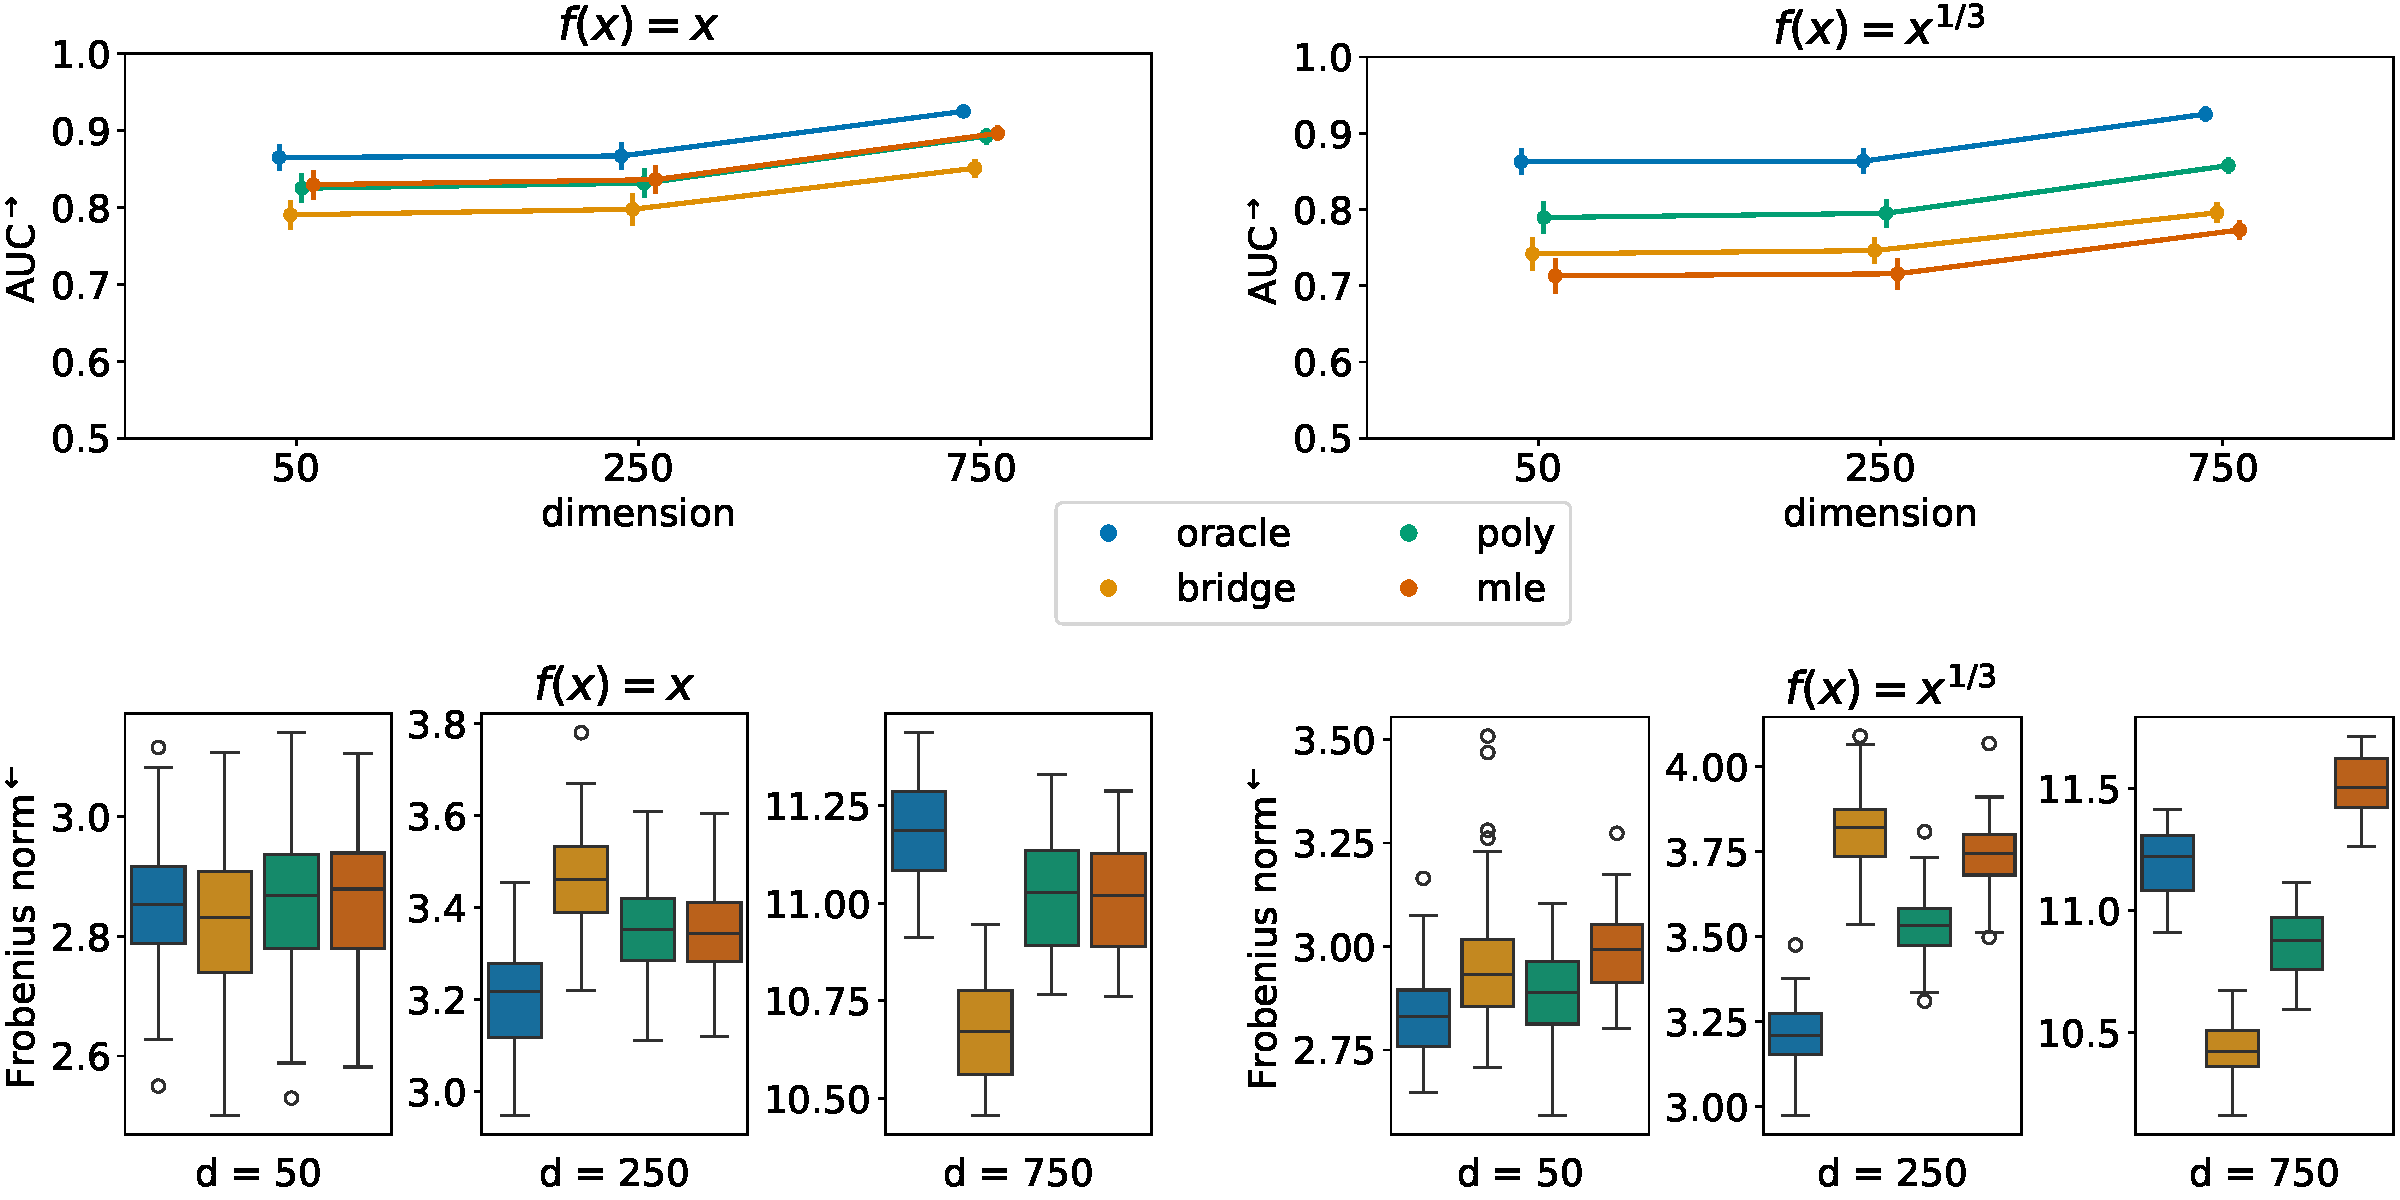
\includegraphics[width=\textwidth]{Figures/simulation_results_general.pdf}
    \caption{Simulation results for the general mixed data setting based on \(100\) simulation runs. The left column corresponds to the latent Gaussian model, where the transformation function is the identity. The right colum depicts results for the LGCM with \(f_j(x) = x^{1/3}\) for all \(j\). The top row reports mean and standard deviation of the AUC along simulation runs, and the bottom row depicts boxplots of the estimation error $\Norm{\hat{\mathbf\Omega} - \mathbf\Omega^*}_F$. The y-axis labels have superscript arrows attached to indicate the direction of improvement: \(\rightarrow\) implies that larger values are better, and \(\leftarrow\) implies that smaller values are better.}
    \label{fig:bench_genral}
\end{figure}

Similar to above, \figref{fig:bench_genral} depicts the mean estimation error $\Norm{\hat{\mathbf\Omega} - \mathbf\Omega^*}_F$ and the AUC and left and right columns correspond to latent Gaussian und LGCM settings, respectively. This time, given general mixed data, differences in terms of AUC between the estimators are noticeable. When the transformations are the identity, the MLE is correctly specified, and it is tied with \texttt{poly} in terms of AUC. The \texttt{bridge} estimator performs worse than the other two estimators. When the transformations are $f_j(x) = x^{1/3}$, the MLE is misspecified, and our \texttt{poly} estimator performs best among non-oracle estimators in terms of AUC. The \texttt{bridge} estimator performs only marginally better than the misspecified \texttt{mle}.

Turning to estimation error results, when \(f_j(x) = x\), the \texttt{poly} and \texttt{mle} estimators perform similarly across dimensions. As the \texttt{oracle} estimator is formed on the latent continuous data, it is unaffected by any discretization and behaves the same as in the binary-continuous case above. The \texttt{bridge} ensemble estimator accounts for a slightly higher estimation error when \(d = 250\) and a lower one when \(d=750\). This pattern can be explained by the FPR of the \texttt{bridge} estimator as illustrated in Figure 4 in the Supplementary Materials. While the FPR is slightly higher in the \(d=250\) case, it is lower in the \(d=750\) case. Similar to the \texttt{oracle} results, this appears to be a consequence of the additional penalty term in the eBIC. Considering the estimation error when \(f_j(x) = x^{1/3}\), the \texttt{poly} and \texttt{bridge} estimators retain their performance. As before, the \texttt{mle} estimator is misspecified and performs worse than the other two estimators.

Overall, the simulation results suggest that our proposed \texttt{poly} estimator performs similarly (binary-continuous data setting) or better (general mixed setting) than the current state-of-the-art. In particular, the \texttt{poly} estimator achieves good performance scores regarding recovery of the graph structure in the general mixed setting. Estimation error results are more sensitive to the choice of the additional high-dimensional penalty. These empirical results suggest that despite the theoretically slower convergence rate, the \texttt{poly} estimator is competitive regarding graph recovery and estimation error.
